\chapter{Embedding Subversion}\label{svn.developer}

Subversion has a modular design: it\textquotesingle s implemented as a
collection of libraries written in C. Each library has a well-defined
purpose and application programming interface (API), and that interface
is available not only for Subversion itself to use, but for any software
that wishes to embed or otherwise programmatically control Subversion.
Additionally, Subversion\textquotesingle s API is available not only to
other C programs, but also to programs written in higher-level languages
such as Python, Perl, Java, and Ruby.

This chapter is for those who wish to interact with Subversion through
its public API or its various language bindings. If you wish to write
robust wrapper scripts around Subversion functionality to simplify your
own life, are trying to develop more complex integrations between
Subversion and other pieces of software, or just have an interest in
Subversion\textquotesingle s various library modules and what they
offer, this chapter is for you. If, however, you don\textquotesingle t
foresee yourself participating with Subversion at such a level, feel
free to skip this chapter with the confidence that your experience as a
Subversion user will not be affected.

\section{Layered Library Design}\label{svn.developer.layerlib}

Each of Subversion\textquotesingle s core libraries can be said to exist
in one of three main layers---the Repository layer, the Repository
Access (RA) layer, or the Client layer (see
\hyperref[svn.intro.architecture.dia-1]{Subversion\textquotesingle s
architecture} in the Preface). We will examine these layers shortly, but
first, let\textquotesingle s briefly summarize
Subversion\textquotesingle s various libraries. For the sake of
consistency, we will refer to the libraries by their extensionless Unix
library names (\texttt{libsvn\_fs}, \texttt{libsvn\_wc},
\texttt{mod\_dav\_svn}, etc.).

\begin{description}
\item[libsvn\_client]
Primary interface for client programs
\item[libsvn\_delta]
Tree and byte-stream differencing routines
\item[libsvn\_diff]
Contextual differencing and merging routines
\item[libsvn\_fs]
Filesystem commons and module loader
\item[libsvn\_fs\_base]
The Berkeley DB filesystem backend
\item[libsvn\_fs\_fs]
The native filesystem (FSFS) backend
\item[libsvn\_ra]
Repository Access commons and module loader
\item[libsvn\_ra\_local]
The local Repository Access module
\item[libsvn\_ra\_serf]
Another (experimental) WebDAV Repository Access module
\item[libsvn\_ra\_svn]
The custom protocol Repository Access module
\item[libsvn\_repos]
Repository interface
\item[libsvn\_subr]
Miscellaneous helpful subroutines
\item[libsvn\_wc]
The working copy management library
\item[mod\_authz\_svn]
Apache authorization module for Subversion repositories access via
WebDAV
\item[mod\_dav\_svn]
Apache module for mapping WebDAV operations to Subversion ones
\end{description}

The fact that the word ``miscellaneous'' appears only once in the
previous list is a good sign. The Subversion development team is serious
about making sure that functionality lives in the right layer and
libraries. Perhaps the greatest advantage of the modular design is its
lack of complexity from a developer\textquotesingle s point of view. As
a developer, you can quickly formulate that kind of ``big picture'' that
allows you to pinpoint the location of certain pieces of functionality
with relative ease.

Another benefit of modularity is the ability to replace a given module
with a whole new library that implements the same API without affecting
the rest of the code base. In some sense, this happens within Subversion
already. The \texttt{libsvn\_ra\_local}, \texttt{libsvn\_ra\_serf}, and
\texttt{libsvn\_ra\_svn} libraries each implement the same interface,
all working as plug-ins to \texttt{libsvn\_ra}. And all three
communicate with the Repository layer---\texttt{libsvn\_ra\_local}
connects to the repository directly; the others do so over a network.
The \texttt{libsvn\_fs\_base} and \texttt{libsvn\_fs\_fs} libraries are
another pair of libraries that implement the same functionality in
different ways---both are plug-ins to the common \texttt{libsvn\_fs}
library.

The client itself also highlights the benefits of modularity in the
Subversion design. Subversion\textquotesingle s \texttt{libsvn\_client}
library is a one-stop shop for most of the functionality necessary for
designing a working Subversion client (see
\hyperref[svn.developer.layerlib.client]{Client Layer}). So while the
Subversion distribution provides only the \texttt{svn} command-line
client program, several third-party programs provide various forms of
graphical client UIs. These GUIs use the same APIs that the stock
command-line client does. This type of modularity has played a large
role in the proliferation of available Subversion clients and IDE
integrations and, by extension, to the tremendous adoption rate of
Subversion itself.

\subsection{Repository Layer}\label{svn.developer.layerlib.repos}

When referring to Subversion\textquotesingle s Repository layer,
we\textquotesingle re generally talking about two basic concepts---the
versioned filesystem implementation (accessed via \texttt{libsvn\_fs},
and supported by its \texttt{libsvn\_fs\_base} and
\texttt{libsvn\_fs\_fs} plug-ins), and the repository logic that wraps
it (as implemented in \texttt{libsvn\_repos}). These libraries provide
the storage and reporting mechanisms for the various revisions of your
version-controlled data. This layer is connected to the Client layer via
the Repository Access layer, and is, from the perspective of the
Subversion user, the stuff at the ``other end of the line.''

The Subversion filesystem is not a kernel-level filesystem that one
would install in an operating system (such as the Linux ext2 or NTFS),
but instead is a virtual filesystem. Rather than storing ``files'' and
``directories'' as real files and directories (the kind you can navigate
through using your favorite shell program), it uses one of two available
abstract storage backends---either a Berkeley DB database environment or
a flat-file representation. (To learn more about the two repository
backends, see \hyperref[svn.reposadmin.basics.backends]{Speaking of
Filesystems\ldots{}}.) There has even been considerable interest by the
development community in giving future releases of Subversion the
ability to use other backend database systems, perhaps through a
mechanism such as Open Database Connectivity (ODBC). In fact, Google did
something similar to this before launching the Google Code Project
Hosting service: they announced in mid-2006 that members of its open
source team had written a new proprietary Subversion filesystem plug-in
that used Google\textquotesingle s ultra-scalable Bigtable database for
its storage.

The filesystem API exported by \texttt{libsvn\_fs} contains the kinds of
functionality you would expect from any other filesystem API---you can
create and remove files and directories, copy and move them around,
modify file contents, and so on. It also has features that are not quite
as common, such as the ability to add, modify, and remove metadata
(``properties'') on each file or directory. Furthermore, the Subversion
filesystem is a versioning filesystem, which means that as you make
changes to your directory tree, Subversion remembers what your tree
looked like before those changes. And before the previous changes. And
the previous ones. And so on, all the way back through versioning time
to (and just beyond) the moment you first started adding things to the
filesystem.

All the modifications you make to your tree are done within the context
of a Subversion commit transaction. The following is a simplified
general routine for modifying your filesystem:

\begin{enumerate}
\def\labelenumi{\arabic{enumi}.}
\item
  Begin a Subversion commit transaction.
\item
  Make your changes (adds, deletes, property modifications, etc.).
\item
  Commit your transaction.
\end{enumerate}

Once you have committed your transaction, your filesystem modifications
are permanently stored as historical artifacts. Each of these cycles
generates a single new revision of your tree, and each revision is
forever accessible as an immutable snapshot of ``the way things were.''

The Transaction Distraction

The notion of a Subversion transaction can become easily confused with
the transaction support provided by the underlying database itself,
especially given the former\textquotesingle s close proximity to the
Berkeley DB database code in \texttt{libsvn\_fs\_base}. Both types of
transaction exist to provide atomicity and isolation. In other words,
transactions give you the ability to perform a set of actions in an
all-or-nothing fashion---either all the actions in the set complete with
success, or they all get treated as though \emph{none} of them ever
happened---and in a way that does not interfere with other processes
acting on the data.

Database transactions generally encompass small operations related
specifically to the modification of data in the database itself (such as
changing the contents of a table row). Subversion transactions are
larger in scope, encompassing higher-level operations such as making
modifications to a set of files and directories that are intended to be
stored as the next revision of the filesystem tree. If that
isn\textquotesingle t confusing enough, consider the fact that
Subversion uses a database transaction during the creation of a
Subversion transaction (so that if the creation of a Subversion
transaction fails, the database will look as though we had never
attempted that creation in the first place)!

Fortunately for users of the filesystem API, the transaction support
provided by the database system itself is hidden almost entirely from
view (as should be expected from a properly modularized library scheme).
It is only when you start digging into the implementation of the
filesystem itself that such things become visible (or interesting).

Most of the functionality the filesystem interface provides deals with
actions that occur on individual filesystem paths. That is, from outside
the filesystem, the primary mechanism for describing and accessing the
individual revisions of files and directories comes through the use of
path strings such as \texttt{/foo/bar}, just as though you were
addressing files and directories through your favorite shell program.
You add new files and directories by passing their paths-to-be to the
right API functions. You query for information about them by the same
mechanism.

Unlike most filesystems, though, a path alone is not enough information
to identify a file or directory in Subversion. Think of a directory tree
as a two-dimensional system, where a node\textquotesingle s siblings
represent a sort of left-and-right motion, and navigating into the
node\textquotesingle s subdirectories represents a downward motion.
\hyperref[svn.developer.layerlib.repos.dia-1]{Files and directories in
two dimensions} shows a typical representation of a tree as exactly
that.

\begin{figure}
\centering
\pandocbounded{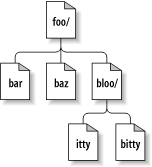
\includegraphics[keepaspectratio]{images/ch08dia1.png}}
\caption{Files and directories in two
dimensions}\label{svn.developer.layerlib.repos.dia-1}
\end{figure}

The difference here is that the Subversion filesystem has a nifty third
dimension that most filesystems do not have---Time!\footnote{We
  understand that this may come as a shock to sci-fi fans who have long
  been under the impression that Time was actually the \emph{fourth}
  dimension, and we apologize for any emotional trauma induced by our
  assertion of a different theory.} In the filesystem interface, nearly
every function that has a \texttt{path} argument also expects a
\texttt{root} argument. This \texttt{svn\_fs\_root\_t} argument
describes either a revision or a Subversion transaction (which is simply
a revision in the making) and provides that third dimension of context
needed to understand the difference between \texttt{/foo/bar} in
revision 32, and the same path as it exists in revision 98.
\hyperref[svn.developer.layerlib.repos.dia-2]{Versioning time---the
third dimension!} shows revision history as an added dimension to the
Subversion filesystem universe.

\begin{figure}
\centering
\pandocbounded{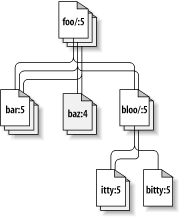
\includegraphics[keepaspectratio]{images/ch08dia2.png}}
\caption{Versioning time---the third
dimension!}\label{svn.developer.layerlib.repos.dia-2}
\end{figure}

As we mentioned earlier, the \texttt{libsvn\_fs} API looks and feels
like any other filesystem, except that it has this wonderful versioning
capability. It was designed to be usable by any program interested in a
versioning filesystem. Not coincidentally, Subversion itself is
interested in that functionality. But while the filesystem API should be
sufficient for basic file and directory versioning support, Subversion
wants more---and that is where \texttt{libsvn\_repos} comes in.

The Subversion repository library (\texttt{libsvn\_repos}) sits
(logically speaking) atop the \texttt{libsvn\_fs} API, providing
additional functionality beyond that of the underlying versioned
filesystem logic. It does not completely wrap each and every filesystem
function---only certain major steps in the general cycle of filesystem
activity are wrapped by the repository interface. Some of these include
the creation and commit of Subversion transactions and the modification
of revision properties. These particular events are wrapped by the
repository layer because they have hooks associated with them. A
repository hook system is not strictly related to implementing a
versioning filesystem, so it lives in the repository wrapper library.

The hooks mechanism is but one of the reasons for the abstraction of a
separate repository library from the rest of the filesystem code. The
\texttt{libsvn\_repos} API provides several other important utilities to
Subversion. These include the abilities to:

\begin{itemize}
\item
  Create, open, destroy, and perform recovery steps on a Subversion
  repository and the filesystem included in that repository.
\item
  Describe the differences between two filesystem trees.
\item
  Query for the commit log messages associated with all (or some) of the
  revisions in which a set of files was modified in the filesystem.
\item
  Generate a human-readable ``dump'' of the filesystem---a complete
  representation of the revisions in the filesystem.
\item
  Parse that dump format, loading the dumped revisions into a different
  Subversion repository.
\end{itemize}

As Subversion continues to evolve, the repository library will grow with
the filesystem library to offer increased functionality and configurable
option support.

\subsection{Repository Access Layer}\label{svn.developer.layerlib.ra}

If the Subversion Repository layer is at ``the other end of the line,''
the Repository Access (RA) layer is the line itself. Charged with
marshaling data between the client libraries and the repository, this
layer includes the \texttt{libsvn\_ra} module loader library, the RA
modules themselves (which currently includes \texttt{libsvn\_ra\_local},
\texttt{libsvn\_ra\_serf}, and \texttt{libsvn\_ra\_svn}), and any
additional libraries needed by one or more of those RA modules (such as
the \texttt{mod\_dav\_svn} Apache module or
\texttt{libsvn\_ra\_svn}\textquotesingle s server, \texttt{svnserve}).

Since Subversion uses URLs to identify its repository resources, the
protocol portion of the URL scheme (usually \texttt{file://},
\texttt{http://}, \texttt{https://}, \texttt{svn://}, or
\texttt{svn+ssh://}) is used to determine which RA module will handle
the communications. Each module registers a list of the protocols it
knows how to ``speak'' so that the RA loader can, at runtime, determine
which module to use for the task at hand. You can determine which RA
modules are available to the Subversion command-line client, and what
protocols they claim to support, by running \texttt{svn\ -\/-version}:

\begin{verbatim}
$ svn --version
svn, version 1.8.0-dev (under development)
   compiled Jan  8 2013, 11:45:25 on i686-pc-linux-gnu

Copyright (C) 2013 The Apache Software Foundation.
This software consists of contributions made by many people;
see the NOTICE file for more information.
Subversion is open source software, see http://subversion.apache.org/

The following repository access (RA) modules are available:

* ra_svn : Module for accessing a repository using the svn network protocol.
  - with Cyrus SASL authentication
  - handles 'svn' scheme
* ra_local : Module for accessing a repository on local disk.
  - handles 'file' scheme
* ra_serf : Module for accessing a repository via WebDAV protocol using serf.
  - handles 'http' scheme
  - handles 'https' scheme

$
\end{verbatim}

The public API exported by the RA layer contains functionality necessary
for sending and receiving versioned data to and from the repository. And
each of the available RA plug-ins is able to perform that task using a
specific protocol---\texttt{libsvn\_ra\_serf} speaks HTTP/WebDAV
(optionally using SSL encryption) with an Apache HTTP Server that is
running the \texttt{mod\_dav\_svn} Subversion server module;
\texttt{libsvn\_ra\_svn} speaks a custom network protocol with the
\texttt{svnserve} program; and so on.

For those who wish to access a Subversion repository using still another
protocol, that is precisely why the Repository Access layer is
modularized! Developers can simply write a new library that implements
the RA interface on one side and communicates with the repository on the
other. Your new library can use existing network protocols or you can
invent your own. You could use interprocess communication (IPC) calls,
or---let\textquotesingle s get crazy, shall we?---you could even
implement an email-based protocol. Subversion supplies the APIs; you
supply the creativity.

\subsection{Client Layer}\label{svn.developer.layerlib.client}

On the client side, the Subversion working copy is where all the action
takes place. The bulk of functionality implemented by the client-side
libraries exists for the sole purpose of managing working
copies---directories full of files and other subdirectories that serve
as a sort of local, editable ``reflection'' of one or more repository
locations---and propagating changes to and from the Repository Access
layer.

Subversion\textquotesingle s working copy library, \texttt{libsvn\_wc},
is directly responsible for managing the data in the working copies. To
accomplish this, the library stores administrative information about the
working copy within a special subdirectory. This subdirectory, named
\texttt{.svn}, is present in each working copy and contains various
other files and directories that record state and provide a private
workspace for administrative action. For those familiar with CVS, this
\texttt{.svn} subdirectory is similar in purpose to the \texttt{CVS}
administrative directories found in CVS working copies.

The Subversion client library, \texttt{libsvn\_client}, has the broadest
responsibility; its job is to mingle the functionality of the working
copy library with that of the Repository Access layer, and then to
provide the highest-level API to any application that wishes to perform
general revision control actions. For example, the function
\texttt{svn\_client\_checkout()} takes a URL as an argument. It passes
this URL to the RA layer and opens an authenticated session with a
particular repository. It then asks the repository for a certain tree,
and sends this tree into the working copy library, which then writes a
full working copy to disk (\texttt{.svn} directories and all).

The client library is designed to be used by any application. While the
Subversion source code includes a standard command-line client, it
should be very easy to write any number of GUI clients on top of the
client library. New GUIs (or any new client, really) for Subversion need
not be clunky wrappers around the included command-line client---they
have full access via the \texttt{libsvn\_client} API to the same
functionality, data, and callback mechanisms that the command-line
client uses. In fact, the Subversion source code tree contains a small C
program (which you can find at
\texttt{tools/examples/minimal\_client.c}) that exemplifies how to wield
the Subversion API to create a simple client program.

Binding Directly---A Word About Correctness

Why should your GUI program bind directly with a \texttt{libsvn\_client}
instead of acting as a wrapper around a command-line program? Besides
simply being more efficient, it can be more correct as well. A
command-line program (such as the one supplied with Subversion) that
binds to the client library needs to effectively translate feedback and
requested data bits from C types to some form of human-readable output.
This type of translation can be lossy. That is, the program may not
display all of the information harvested from the API or may combine
bits of information for compact representation.

If you wrap such a command-line program with yet another program, the
second program has access only to already interpreted (and as we
mentioned, likely incomplete) information, which it must \emph{again}
translate into \emph{its} representation format. With each layer of
wrapping, the integrity of the original data is potentially tainted more
and more, much like the result of making a copy of a copy (of a
copy\ldots) of a favorite audio or video cassette.

But the most compelling argument for binding directly to the APIs
instead of wrapping other programs is that the Subversion project makes
compatibility promises regarding its APIs. Across minor versions of
those APIs (such as between 1.3 and 1.4), no function\textquotesingle s
prototype will change. In other words, you aren\textquotesingle t forced
to update your program\textquotesingle s source code simply because
you\textquotesingle ve upgraded to a new version of Subversion. Certain
functions might be deprecated, but they still work, and this gives you a
buffer of time to eventually embrace the newer APIs. These kinds of
compatibility promises do not exist for Subversion command-line program
output, which is subject to change from release to release.

\section{Using the APIs}\label{svn.developer.usingapi}

Developing applications against the Subversion library APIs is fairly
straightforward. Subversion is primarily a set of C libraries, with
header (\texttt{.h}) files that live in the \texttt{subversion/include}
directory of the source tree. These headers are copied into your system
locations (e.g., \texttt{/usr/local/include}) when you build and install
Subversion itself from source. These headers represent the entirety of
the functions and types meant to be accessible by users of the
Subversion libraries. The Subversion developer community is meticulous
about ensuring that the public API is well documented---refer directly
to the header files for that documentation.

When examining the public header files, the first thing you might notice
is that Subversion\textquotesingle s datatypes and functions are
namespace-protected. That is, every public Subversion symbol name begins
with \texttt{svn\_}, followed by a short code for the library in which
the symbol is defined (such as \texttt{wc}, \texttt{client},
\texttt{fs}, etc.), followed by a single underscore (\texttt{\_}), and
then the rest of the symbol name. Semipublic functions (used among
source files of a given library but not by code outside that library,
and found inside the library directories themselves) differ from this
naming scheme in that instead of a single underscore after the library
code, they use a double underscore (\texttt{\_\ \_}). Functions that are
private to a given source file have no special prefixing and are
declared \texttt{static}. Of course, a compiler isn\textquotesingle t
interested in these naming conventions, but they help to clarify the
scope of a given function or datatype.

Another good source of information about programming against the
Subversion APIs is the project\textquotesingle s own hacking guidelines,
which you can find at
\href{https://subversion.apache.org/docs/community-guide/}{}. This
document contains useful information, which, while aimed at developers
and would-be developers of Subversion itself, is equally applicable to
folks developing against Subversion as a set of third-party
libraries.\footnote{After all, Subversion uses
  Subversion\textquotesingle s APIs, too.}

\subsection{The Apache Portable Runtime
Library}\label{svn.developer.usingapi.apr}

Along with Subversion\textquotesingle s own datatypes, you will see many
references to datatypes that begin with \texttt{apr\_}---symbols from
the Apache Portable Runtime (APR) library. APR is
Apache\textquotesingle s portability library, originally carved out of
its server code as an attempt to separate the OS-specific bits from the
OS-independent portions of the code. The result was a library that
provides a generic API for performing operations that differ mildly---or
wildly---from OS to OS. While the Apache HTTP Server was obviously the
first user of the APR library, the Subversion developers immediately
recognized the value of using APR as well. This means that there is
practically no OS-specific code in Subversion itself. Also, it means
that the Subversion client compiles and runs anywhere that the Apache
HTTP Server does. Currently, this list includes all flavors of Unix,
Win32, BeOS, OS/2, and Mac OS X.

In addition to providing consistent implementations of system calls that
differ across operating systems,\footnote{Subversion uses ANSI system
  calls and datatypes as much as possible.} APR gives Subversion
immediate access to many custom datatypes, such as dynamic arrays and
hash tables. Subversion uses these types extensively. But perhaps the
most pervasive APR datatype, found in nearly every Subversion API
prototype, is the \texttt{apr\_pool\_t}---the APR memory pool.
Subversion uses pools internally for all its memory allocation needs
(unless an external library requires a different memory management
mechanism for data passed through its API),\footnote{Berkeley DB is an
  example of such a library.} and while a person coding against the
Subversion APIs is not required to do the same, she \emph{is} required
to provide pools to the API functions that need them. This means that
users of the Subversion API must also link against APR, must call
\texttt{apr\_initialize()} to initialize the APR subsystem, and then
must create and manage pools for use with Subversion API calls,
typically by using \texttt{svn\_pool\_create()},
\texttt{svn\_pool\_clear()}, and \texttt{svn\_pool\_destroy()}.

Programming with Memory Pools

Almost every developer who has used the C programming language has at
some point sighed at the daunting task of managing memory usage.
Allocating enough memory to use, keeping track of those allocations,
freeing the memory when you no longer need it---these tasks can be quite
complex. And of course, failure to do those things properly can result
in a program that crashes itself, or worse, crashes the computer.

Higher-level languages, on the other hand, either take the job of memory
management away from you completely or make it something you toy with
only when doing extremely tight program optimization. Languages such as
Java and Python use garbage collection, allocating memory for objects
when needed, and automatically freeing that memory when the object is no
longer in use.

APR provides a middle-ground approach called pool-based memory
management. It allows the developer to control memory usage at a lower
resolution---per chunk (or ``pool'') of memory, instead of per allocated
object. Rather than using \texttt{malloc()} and friends to allocate
enough memory for a given object, you ask APR to allocate the memory
from a memory pool. When you\textquotesingle re finished using the
objects you\textquotesingle ve created in the pool, you destroy the
entire pool, effectively de-allocating the memory consumed by \emph{all}
the objects you allocated from it. Thus, rather than keeping track of
individual objects that need to be de-allocated, your program simply
considers the general lifetimes of those objects and allocates the
objects in a pool whose lifetime (the time between the
pool\textquotesingle s creation and its deletion) matches the
object\textquotesingle s needs.

\subsection{Functions and
Batons}\label{svn.developer.usingapi.funcsbatons}

To facilitate ``streamy'' (asynchronous) behavior and provide consumers
of the Subversion C API with hooks for handling information in
customizable ways, many functions in the API accept pairs of parameters:
a pointer to a callback function, and a pointer to a blob of memory
called a baton that carries context information for that callback
function. Batons are typically C structures with additional information
that the callback function needs but which is not given directly to the
callback function by the driving API function.

\subsection{URL and Path
Requirements}\label{svn.developer.usingapi.urlpath}

With remote version control operation as the whole point of
Subversion\textquotesingle s existence, it makes sense that some
attention has been paid to internationalization (i18n) support. After
all, while ``remote'' might mean ``across the office,'' it could just as
well mean ``across the globe.'' To facilitate this, all of
Subversion\textquotesingle s public interfaces that accept path
arguments expect those paths to be canonicalized---which is most easily
accomplished by passing them through
\texttt{svn\_dirent\_canonicalize()} or
\texttt{svn\_uri\_canonicalize()} (depending on whether you are
canonicalizing a local system path or a URL, respectively)---and encoded
in UTF-8. This means, for example, that any new client binary that
drives the \texttt{libsvn\_client} interface needs to first convert
paths from the locale-specific encoding to UTF-8 before passing those
paths to the Subversion libraries, and then reconvert any resultant
output paths from Subversion back into the locale\textquotesingle s
encoding before using those paths for non-Subversion purposes.
Fortunately, Subversion provides a suite of functions (see
\texttt{subversion/include/svn\_utf.h}) that any program can use to do
these conversions.

Also, Subversion APIs require all URL parameters to be properly
URI-encoded. So, instead of passing
\url{file:///home/username/My\%C2\%A0File.txt} as the URL of a file
named \texttt{My\ File.txt}, you need to pass
\url{file:///home/username/My\%20File.txt}. Again, Subversion supplies
helper functions that your application can
use---\texttt{svn\_path\_uri\_encode()} and
\texttt{svn\_path\_uri\_decode()}, for URI encoding and decoding,
respectively.

\subsection{Using Languages Other Than C and
C++}\label{svn.developer.usingapi.otherlangs}

If you are interested in using the Subversion libraries in conjunction
with something other than a C program---say, a Python or Perl
script---Subversion has some support for this via the Simplified Wrapper
and Interface Generator (SWIG). The SWIG bindings for Subversion are
located in \texttt{subversion/bindings/swig}. They are still maturing,
but they are usable. These bindings allow you to call Subversion API
functions indirectly, using wrappers that translate the datatypes native
to your scripting language into the datatypes needed by
Subversion\textquotesingle s C libraries.

Significant efforts have been made toward creating functional
SWIG-generated bindings for Python, Perl, and Ruby. To some extent, the
work done preparing the SWIG interface files for these languages is
reusable in efforts to generate bindings for other languages supported
by SWIG (which include versions of C\#, Guile, Java, MzScheme, OCaml,
PHP, and Tcl, among others). However, some extra programming is required
to compensate for complex APIs that SWIG needs some help translating
between languages. For more information on SWIG itself, see the
project\textquotesingle s web site at \href{https://www.swig.org/}{}.

Subversion also has language bindings for Java. The javahl bindings
(located in \texttt{subversion/bindings/java} in the Subversion source
tree) aren\textquotesingle t SWIG-based, but are instead a mixture of
Java and hand-coded JNI. Javahl covers most Subversion client-side APIs
and is specifically targeted at implementors of Java-based Subversion
clients and IDE integrations.

Subversion\textquotesingle s language bindings tend to lack the level of
developer attention given to the core Subversion modules, but can
generally be trusted as production-ready. A number of scripts and
applications, alternative Subversion GUI clients, and other third-party
tools are successfully using Subversion\textquotesingle s language
bindings today to accomplish their Subversion integrations.

It\textquotesingle s worth noting here that there are other options for
interfacing with Subversion using other languages: alternative bindings
for Subversion that aren\textquotesingle t provided by the Subversion
development community at all. There are a couple of popular ones we feel
are especially noteworthy. First, Barry Scott\textquotesingle s PySVN
bindings (\href{https://pysvn.sourceforge.io/}{}) are a popular option
for binding with Python. PySVN boasts of a more Pythonic interface than
the more C-like APIs provided by Subversion\textquotesingle s own Python
bindings. And if you\textquotesingle re looking for a pure Java
implementation of Subversion, check out SVNKit
(\href{https://svnkit.com/}{}), which is Subversion rewritten from the
ground up in Java.

SVNKit Versus javahl

In 2005, a small company called TMate announced the 1.0.0 release of
JavaSVN---a pure Java implementation of Subversion. Since then, the
project has been renamed to SVNKit (available at
\href{https://svnkit.com/}{}) and has seen great success as a provider
of Subversion functionality to various Subversion clients, IDE
integrations, and other third-party tools.

The SVNKit library is interesting in that, unlike the javahl library, it
is not merely a wrapper around the official Subversion core libraries.
In fact, it shares no code with Subversion at all. But while it is easy
to confuse SVNKit with javahl, and easier still to not even realize
which of these libraries you are using, folks should be aware that
SVNKit differs from javahl in some significant ways. First, while SVNKit
is developed as open source software just like Subversion,
SVNKit\textquotesingle s license is more restrictive than that of
Subversion.\footnote{Redistributions in any form must be accompanied by
  information on how to obtain complete source code for the software
  that uses SVNKit and any accompanying software that uses the software
  that uses SVNKit. See \href{https://svnkit.com/license.html}{} for
  details.} Finally, by aiming to be a pure Java Subversion library,
SVNKit is limited in which portions of Subversion can be reasonably
cloned while still keeping up with Subversion\textquotesingle s
releases. This has already happened once---SVNKit cannot access
BDB-backed Subversion repositories via the \texttt{file://} protocol
because there\textquotesingle s no pure Java implementation of Berkeley
DB that is file-format-compatible with the native implementation of that
library.

That said, SVNKit has a well-established track record of reliability.
And a pure Java solution is much more robust in the face of programming
errors---a bug in SVNKit might raise a catchable Java Exception, but a
bug in the Subversion core libraries as accessed via javahl can bring
down your entire Java Runtime Environment. So, weigh the costs when
choosing a Java-based Subversion implementation.

\subsection{Code Samples}\label{svn.developer.usingapi.codesamples}

\hyperref[svn.developer.layerlib.repos.ex-1]{Using the repository layer}
contains a code segment (written in C) that illustrates some of the
concepts we\textquotesingle ve been discussing. It uses both the
repository and filesystem interfaces (as can be determined by the
prefixes \texttt{svn\_repos\_} and \texttt{svn\_fs\_} of the function
names, respectively) to create a new revision in which a directory is
added. You can see the use of an APR pool, which is passed around for
memory allocation purposes. Also, the code reveals a somewhat obscure
fact about Subversion error handling---all Subversion errors must be
explicitly handled to avoid memory leakage (and in some cases,
application failure).

\protect\phantomsection\label{svn.developer.layerlib.repos.ex-1}
Using the repository layer

\begin{verbatim}
/* Convert a Subversion error into a simple boolean error code.
 *
 * NOTE:  Subversion errors must be cleared (using svn_error_clear())
 *        because they are allocated from the global pool, else memory
 *        leaking occurs.
 */
#define INT_ERR(expr)                           \
  do {                                          \
    svn_error_t *__temperr = (expr);            \
    if (__temperr)                              \
      {                                         \
        svn_error_clear(__temperr);             \
        return 1;                               \
      }                                         \
    return 0;                                   \
  } while (0)

/* Create a new directory at the path NEW_DIRECTORY in the Subversion
 * repository located at REPOS_PATH.  Perform all memory allocation in
 * POOL.  This function will create a new revision for the addition of
 * NEW_DIRECTORY.  Return zero if the operation completes
 * successfully, nonzero otherwise.
 */
static int
make_new_directory(const char *repos_path,
                   const char *new_directory,
                   apr_pool_t *pool)
{
  svn_error_t *err;
  svn_repos_t *repos;
  svn_fs_t *fs;
  svn_revnum_t youngest_rev;
  svn_fs_txn_t *txn;
  svn_fs_root_t *txn_root;
  const char *conflict_str;

  /* Open the repository located at REPOS_PATH. 
   */
  INT_ERR(svn_repos_open(&repos, repos_path, pool));

  /* Get a pointer to the filesystem object that is stored in REPOS. 
   */
  fs = svn_repos_fs(repos);

  /* Ask the filesystem to tell us the youngest revision that
   * currently exists. 
   */
  INT_ERR(svn_fs_youngest_rev(&youngest_rev, fs, pool));

  /* Begin a new transaction that is based on YOUNGEST_REV.  We are
   * less likely to have our later commit rejected as conflicting if we
   * always try to make our changes against a copy of the latest snapshot
   * of the filesystem tree. 
   */
  INT_ERR(svn_repos_fs_begin_txn_for_commit2(&txn, repos, youngest_rev,
                                             apr_hash_make(pool), pool));

  /* Now that we have started a new Subversion transaction, get a root
   * object that represents that transaction. 
   */
  INT_ERR(svn_fs_txn_root(&txn_root, txn, pool));
  
  /* Create our new directory under the transaction root, at the path
   * NEW_DIRECTORY. 
   */
  INT_ERR(svn_fs_make_dir(txn_root, new_directory, pool));

  /* Commit the transaction, creating a new revision of the filesystem
   * which includes our added directory path.
   */
  err = svn_repos_fs_commit_txn(&conflict_str, repos, 
                                &youngest_rev, txn, pool);
  if (! err)
    {
      /* No error?  Excellent!  Print a brief report of our success.
       */
      printf("Directory '%s' was successfully added as new revision "
             "'%ld'.\n", new_directory, youngest_rev);
    }
  else if (err->apr_err == SVN_ERR_FS_CONFLICT)
    {
      /* Uh-oh.  Our commit failed as the result of a conflict
       * (someone else seems to have made changes to the same area 
       * of the filesystem that we tried to modify).  Print an error
       * message.
       */
      printf("A conflict occurred at path '%s' while attempting "
             "to add directory '%s' to the repository at '%s'.\n", 
             conflict_str, new_directory, repos_path);
    }
  else
    {
      /* Some other error has occurred.  Print an error message.
       */
      printf("An error occurred while attempting to add directory '%s' "
             "to the repository at '%s'.\n", 
             new_directory, repos_path);
    }

  INT_ERR(err);
} 
\end{verbatim}

Note that in \hyperref[svn.developer.layerlib.repos.ex-1]{Using the
repository layer}, the code could just as easily have committed the
transaction using \texttt{svn\_fs\_commit\_txn()}. But the filesystem
API knows nothing about the repository library\textquotesingle s hook
mechanism. If you want your Subversion repository to automatically
perform some set of non-Subversion tasks every time you commit a
transaction (e.g., sending an email that describes all the changes made
in that transaction to your developer mailing list), you need to use the
\texttt{libsvn\_repos}-wrapped version of that function, which adds the
hook triggering functionality---in this case,
\texttt{svn\_repos\_fs\_commit\_txn()}. (For more information regarding
Subversion\textquotesingle s repository hooks, see
\hyperref[svn.reposadmin.hooks]{Implementing Repository Hooks}.)

Now let\textquotesingle s switch languages.
\hyperref[svn.developer.usingapi.otherlangs.ex-1]{Using the repository
layer with Python} is a sample program that uses
Subversion\textquotesingle s SWIG Python bindings to recursively crawl
the youngest repository revision, and to print the various paths reached
during the crawl.

\protect\phantomsection\label{svn.developer.usingapi.otherlangs.ex-1}
Using the repository layer with Python

\begin{verbatim}
#!/usr/bin/python

"""Crawl a repository, printing versioned object path names."""

import sys
import os.path
import svn.fs, svn.core, svn.repos

def crawl_filesystem_dir(root, directory):
    """Recursively crawl DIRECTORY under ROOT in the filesystem, and return
    a list of all the paths at or below DIRECTORY."""

    # Print the name of this path.
    print directory + "/"
    
    # Get the directory entries for DIRECTORY.
    entries = svn.fs.svn_fs_dir_entries(root, directory)

    # Loop over the entries.
    names = entries.keys()
    for name in names:
        # Calculate the entry's full path.
        full_path = directory + '/' + name

        # If the entry is a directory, recurse.  The recursion will return
        # a list with the entry and all its children, which we will add to
        # our running list of paths.
        if svn.fs.svn_fs_is_dir(root, full_path):
            crawl_filesystem_dir(root, full_path)
        else:
            # Else it's a file, so print its path here.
            print full_path

def crawl_youngest(repos_path):
    """Open the repository at REPOS_PATH, and recursively crawl its
    youngest revision."""
    
    # Open the repository at REPOS_PATH, and get a reference to its
    # versioning filesystem.
    repos_obj = svn.repos.svn_repos_open(repos_path)
    fs_obj = svn.repos.svn_repos_fs(repos_obj)

    # Query the current youngest revision.
    youngest_rev = svn.fs.svn_fs_youngest_rev(fs_obj)
    
    # Open a root object representing the youngest (HEAD) revision.
    root_obj = svn.fs.svn_fs_revision_root(fs_obj, youngest_rev)

    # Do the recursive crawl.
    crawl_filesystem_dir(root_obj, "")
    
if __name__ == "__main__":
    # Check for sane usage.
    if len(sys.argv) != 2:
        sys.stderr.write("Usage: %s REPOS_PATH\n"
                         % (os.path.basename(sys.argv[0])))
        sys.exit(1)

    # Canonicalize the repository path.
    repos_path = svn.core.svn_dirent_canonicalize(sys.argv[1])

    # Do the real work.
    crawl_youngest(repos_path)
\end{verbatim}

This same program in C would need to deal with APR\textquotesingle s
memory pool system. But Python handles memory usage automatically, and
Subversion\textquotesingle s Python bindings adhere to that convention.
In C, you\textquotesingle d be working with custom datatypes (such as
those provided by the APR library) for representing the hash of entries
and the list of paths, but Python has hashes (called ``dictionaries'')
and lists as built-in datatypes, and it provides a rich collection of
functions for operating on those types. So SWIG (with the help of some
customizations in Subversion\textquotesingle s language bindings layer)
takes care of mapping those custom datatypes into the native datatypes
of the target language. This provides a more intuitive interface for
users of that language.

The Subversion Python bindings can be used for working copy operations,
too. In the previous section of this chapter, we mentioned the
\texttt{libsvn\_client} interface and how it exists for the sole purpose
of simplifying the process of writing a Subversion client.
\hyperref[svn.developer.usingapi.otherlangs.ex-2]{A Python status
crawler} is a brief example of how that library can be accessed via the
SWIG Python bindings to re-create a scaled-down version of the
\texttt{svn\ status} command.

\protect\phantomsection\label{svn.developer.usingapi.otherlangs.ex-2}
A Python status crawler

\begin{verbatim}
#!/usr/bin/env python

"""Crawl a working copy directory, printing status information."""

import sys
import os.path
import getopt
import svn.core, svn.client, svn.wc

def generate_status_code(status):
    """Translate a status value into a single-character status code,
    using the same logic as the Subversion command-line client."""
    code_map = { svn.wc.svn_wc_status_none        : ' ',
                 svn.wc.svn_wc_status_normal      : ' ',
                 svn.wc.svn_wc_status_added       : 'A',
                 svn.wc.svn_wc_status_missing     : '!',
                 svn.wc.svn_wc_status_incomplete  : '!',
                 svn.wc.svn_wc_status_deleted     : 'D',
                 svn.wc.svn_wc_status_replaced    : 'R',
                 svn.wc.svn_wc_status_modified    : 'M',
                 svn.wc.svn_wc_status_conflicted  : 'C',
                 svn.wc.svn_wc_status_obstructed  : '~',
                 svn.wc.svn_wc_status_ignored     : 'I',
                 svn.wc.svn_wc_status_external    : 'X',
                 svn.wc.svn_wc_status_unversioned : '?',
               }
    return code_map.get(status, '?')

def do_status(wc_path, verbose, prefix):
    # Build a client context baton.
    ctx = svn.client.svn_client_create_context()

    def _status_callback(path, status):
        """A callback function for svn_client_status."""

        # Print the path, minus the bit that overlaps with the root of
        # the status crawl
        text_status = generate_status_code(status.text_status)
        prop_status = generate_status_code(status.prop_status)
        prefix_text = ''
        if prefix is not None:
            prefix_text = prefix + " "
        print '%s%s%s  %s' % (prefix_text, text_status, prop_status, path)
        
    # Do the status crawl, using _status_callback() as our callback function.
    revision = svn.core.svn_opt_revision_t()
    revision.type = svn.core.svn_opt_revision_head
    svn.client.svn_client_status2(wc_path, revision, _status_callback,
                                  svn.core.svn_depth_infinity, verbose,
                                  0, 0, 1, ctx)

def usage_and_exit(errorcode):
    """Print usage message, and exit with ERRORCODE."""
    stream = errorcode and sys.stderr or sys.stdout
    stream.write("""Usage: %s OPTIONS WC-PATH

  Print working copy status, optionally with a bit of prefix text.

Options:
  --help, -h    : Show this usage message
  --prefix ARG  : Print ARG, followed by a space, before each line of output
  --verbose, -v : Show all statuses, even uninteresting ones
""" % (os.path.basename(sys.argv[0])))
    sys.exit(errorcode)
    
if __name__ == '__main__':
    # Parse command-line options.
    try:
        opts, args = getopt.getopt(sys.argv[1:], "hv",
                                   ["help", "prefix=", "verbose"])
    except getopt.GetoptError:
        usage_and_exit(1)
    verbose = 0
    prefix = None
    for opt, arg in opts:
        if opt in ("-h", "--help"):
            usage_and_exit(0)
        if opt in ("--prefix"):
            prefix = arg
        if opt in ("-v", "--verbose"):
            verbose = 1
    if len(args) != 1:
        usage_and_exit(2)
            
    # Canonicalize the working copy path.
    wc_path = svn.core.svn_dirent_canonicalize(args[0])

    # Do the real work.
    try:
        do_status(wc_path, verbose, prefix)
    except svn.core.SubversionException, e:
        sys.stderr.write("Error (%d): %s\n" % (e.apr_err, e.message))
        sys.exit(1)
\end{verbatim}

As was the case in
\hyperref[svn.developer.usingapi.otherlangs.ex-1]{Using the repository
layer with Python}, this program is pool-free and uses, for the most
part, normal Python datatypes.

Run user-provided paths through the appropriate canonicalization
function (\texttt{svn\_dirent\_canonicalize()} or
\texttt{svn\_uri\_canonicalize()}) before passing them to other API
functions. Failure to do so can trigger assertions in the underlying
Subversion C library which translate into rather immediate and
unceremonious program abortion.

Of particular interest to users of the Python flavor of
Subversion\textquotesingle s API is the implementation of callback
functions. As previously mentioned, Subversion\textquotesingle s C API
makes liberal use of the callback function/baton paradigm. API functions
which in C accept a function and baton pair only accept a callback
function parameter in Python. How, then, does the caller pass arbitrary
context information to the callback function? In Python, this is done by
taking advantage of Python\textquotesingle s scoping rules and default
argument values. You can see this in action in
\hyperref[svn.developer.usingapi.otherlangs.ex-2]{A Python status
crawler}. The \texttt{svn\_client\_status2()} function is given a
callback function (\texttt{\_status\_callback()}) but no
baton---\texttt{\_status\_callback()} gets access to the user-provided
prefix string because that variable falls into the scope of the function
automatically.

\section{Summary}\label{svn.developer.summary}

One of Subversion\textquotesingle s greatest features
isn\textquotesingle t something you get from running its command-line
client or other tools. It\textquotesingle s the fact that Subversion was
designed modularly and provides a stable, public API so that
others---like yourself, perhaps---can write custom software that drives
Subversion\textquotesingle s core logic.

In this chapter, we took a closer look at Subversion\textquotesingle s
architecture, examining its logical layers and describing that public
API, the very same API that Subversion\textquotesingle s own layers use
to communicate with each other. Many developers have found interesting
uses for the Subversion API, from simple repository hook scripts, to
integrations between Subversion and some other application, to
completely different version control systems. What unique itch will
\emph{you} scratch with it?

